\section{\textbf{Dependencies in Dyadic Data}}

In thinking about dyadic data, scholars in the field begin by structuring it as a set of dyadic observations stacked on top of one another. Each observation is assumed to be independent of the others. Thus, for example, a conflict sent from actor the United States to Japan, is assumed to be independent of any action that Japan may send to the United States. Additionally, every action sent by Japan to others in the system is considered independent even though each of those interactions involves a common sender, i.e, Japan. As a result, the assumption that most begin with is that each dyadic interaction is taking place in isolation of the others. 

\begin{table}[ht]
	\captionsetup{justification=raggedright }
	\centering
	\begin{minipage}{.45\textwidth}
		\centering
		\begingroup
		\setlength{\tabcolsep}{10pt}
		\begin{tabular}{ccc}
			Sender & Receiver & Event \\
			\hline\hline
			$i$ & $j$ & $y_{ij}$ \\
			\multirow{2}{*}{\vdots} & $k$ & $y_{ik}$ \\
			~ & $l$ & $y_{il}$ \\
			$j$ & $i$ & $y_{ji}$ \\
			\multirow{2}{*}{\vdots} & $k$ & $y_{jk}$ \\
			~ & $l$ & $y_{jl}$ \\
			$k$ & $i$ & $y_{ki}$ \\
			\multirow{2}{*}{\vdots} & $j$ & $y_{kj}$ \\
			~ & $l$ & $y_{kl}$ \\
			$l$ & $i$ & $y_{li}$ \\
			\multirow{2}{*}{\vdots} & $j$ & $y_{lj}$ \\
			~ & $k$ & $y_{lk}$ \\
			\hline\hline
		\end{tabular}
		\endgroup
		\caption{Structure of datasets used in canonical design.} 
		\label{tab:canDesign}
	\end{minipage}
	$\mathbf{\longrightarrow}$
	\begin{minipage}{.45\textwidth}
		\centering
		\begingroup
		\setlength{\tabcolsep}{10pt}
		\renewcommand{\arraystretch}{1.5}
		\begin{tabular}{c||cccc}
		~ & $i$ & $j$ & $k$ & $l$ \\ \hline\hline
		$i$ & \footnotesize{NA} & $y_{ij}$ & $y_{ik}$ & $y_{il}$ \\
		$j$ & $y_{ji}$ & \footnotesize{NA}  & $y_{jk}$ & $y_{jl}$ \\
		$k$ & $y_{ki}$ & $y_{kj}$ & \footnotesize{NA}  & $y_{kl}$ \\
		$l$ & $y_{li}$ & $y_{lj}$ & $y_{lk}$ & \footnotesize{NA}  \\
		\end{tabular}
		\endgroup
		\caption{Adjacency matrix representation of data in Table~\ref{tab:canDesign}. Senders are represented by the rows and receivers by the columns. }
		\label{tab:netDesign}
	\end{minipage}
\end{table}

\FloatBarrier

To start to move away from this assumption and better understand the dependencies that emerge in relational data it is helpful to shift towards structuring dyadic data in the form of an adjacency matrix as shown in the top right of Table~\ref{tab:netDesign}. Here rows designate the senders of an event and columns the receivers. The cross-sections in this matrix represent the action that was sent by an actor on the row to one designated in the column. Thus $y_{ij}$ designates an action, such as a conflictual event or trade flows, that is sent from actor $i$ to actor $j$. 

Using the structure of an adjacency matrix we can visualize the types of first and second order dependencies that complicate the analysis of relational data in traditional GLMs. Figure~\ref{fig:adjMatDeps} clarifies the types of dependencies that can manifest in these types of data structures. The adjacency matrix on the top left highlights a particular row of an adjacency matrix, to illustrate that values across a particular row of an adjacency matrix may be more similar to each other than other values in the adjacency matrix because each of these values has a common sender. Homogeneity in interactions involving a common sender also manifest heterogeneity in how active actors are across the network when compared to each other. Thus in most relational datasets (e.g., trade flows, conflict, participation in international organizations, even networks derived from Twitter or Facebook) we often find that there are some actors who are much more active than others \citep{barabasi:reka:1999}. Unless one is able to develop a model that can account for the variety of explanations that may play a role in determining why a particular actor may be more active than others, parameter estimates from standard statistical models will be biased.

\begin{figure}
	\begin{tabular}{cc}
		\texttt{Sender heterogeneity} & \texttt{Receiver Heterogeneity} \\
		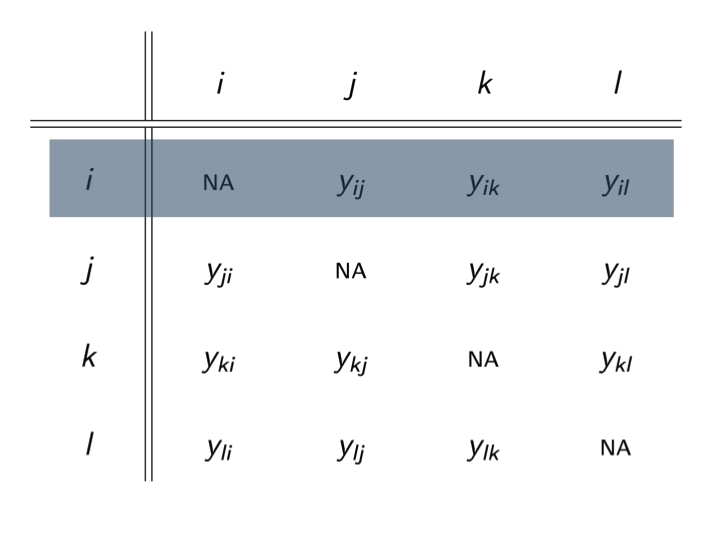
\includegraphics[width=.45\textwidth]{adjRowDep.png} & 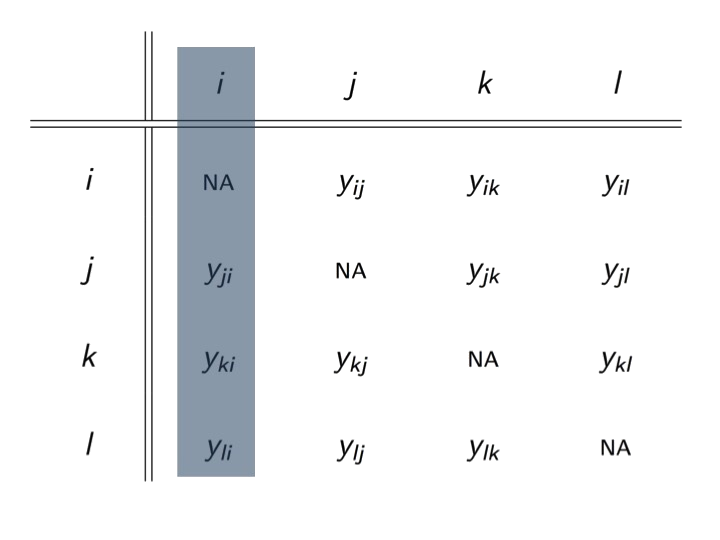
\includegraphics[width=.45\textwidth]{adjColDep.png} \\
		\texttt{Sender-Receiver Covariance} & \texttt{Reciprocity} \\
		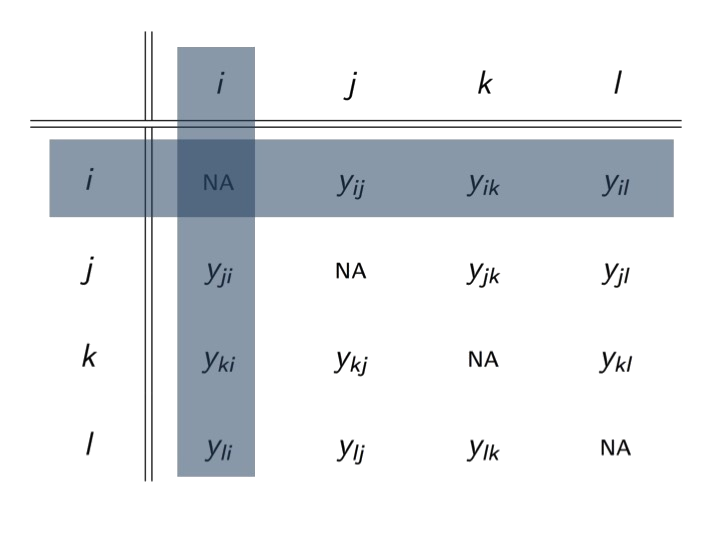
\includegraphics[width=.45\textwidth]{adjRowColCovar.png} & 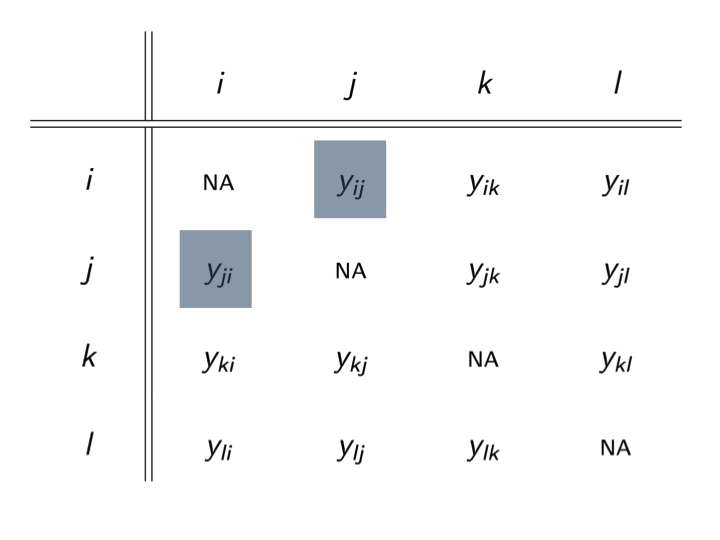
\includegraphics[width=.45\textwidth]{adjRecip.png} \\
	\end{tabular}
	\caption{Nodal and dyadic dependencies in relational data.}
	\label{fig:adjMatDeps}
\end{figure}

For similar reasons one also needs to take into account that there is a shared dependence between dyadic observations that share a common receiver. The bottom-left panel, illustrates that sender and receiver type dependencies can also blend together. Specifically, as actors who are more likely to send ties in a network tend to also be more likely to receive them. As a result, the rows and columns in an adjacency matrix are often correlated. For example, consider that trade flows both from and to many wealthy, developed countries. The bottom-right panel, highlights a second order dependence, specifically, reciprocity. This is a dependency occurring within dyads involving the same actors whereby values of $y_{ij}$ and $y_{ji}$ are correlated. The concept of reciprocity has deep roots in the study of relations between states \citep{richardson:1960,keohane:1989}. The purpose of highlighting each of these dependencies through the set of panels in Figure~\ref{fig:adjMatDeps} is to more easily visualize how each of these dependencies manifest in relational data. Alternatively, when we simply simply stack dyads in some arbitrary order, these dependencies are easy to ignore.

The dependencies discussed so far involve at most dependence between two actors. For most relational data, however, dependencies do not simply manifest at this level. More often we find significant evidence of higher order structures that result from dependencies between multiple groups of actors. These dependencies arise because there may be a or some set of latent attributes between actors that affects their probability of interacting with one another \citep{wasserman:faust:1994,zinnes:1967}. In Figure~\ref{fig:thirdDeps} we provide a visualization of a hypothetical relational dataset. Here the nodes designate actors and edges between the nodes indicate that an interaction between the two took place. Each node is colored by the latent group to which they belong. 

\begin{figure}[ht]
	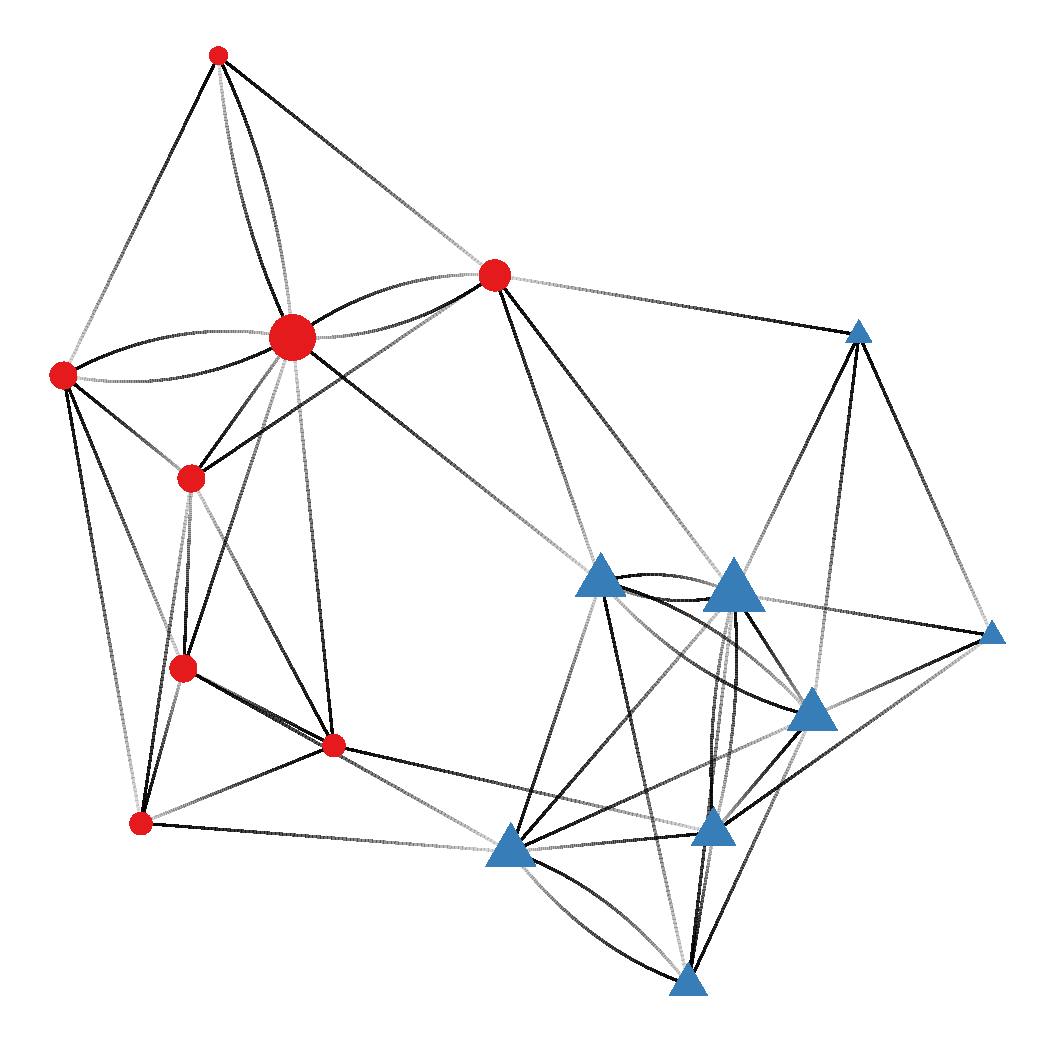
\includegraphics[width=.7\textwidth]{stochEquiv.pdf}
	\caption{Visualization of network with meso-scopic features.}
	\label{fig:thirdDeps}
\end{figure}

Clear from the visualization is that the actors belonging to the same group have a higher likelihood of having an interaction with each other than those from the other group. A prominent example of a network with this type of structure was found by \citet{adamic:glance:2005}, who visualized the ways in which right and left leaning political blogs linked to one another in the 2004 United States Election \citep{adamic:glance:2005}. They found that the degree of interaction between right and left leaning blogs was minimal, and that most of these blogs simply linked to those of their own ilk. This showcases the types of higher order dependencies that can emerge in relational data. First, the fact that interactions was determined by a shared attribute, in this case political ideology, is an example of homophily. Homophily can be used to explain the emergence of patterns such as transitivity (``a friend of a friend is a friend'') and balance (``an enemy of a friend is an enemy''), which also have a long history in international relations. The other major type of meso-scopic feature that emerges in relational data is community structure, which is often formalized through the concept of stochastic equivalence \citep{anderson:etal:1992}. This concept simply refers to the idea that groups of nodes that act similarly in the network are stochastically equivalent. In the example we have laid out above each of the left leaning blogs would be considered stochastically equivalent to one another. 

The major implication of the presence of homophily, stochastic equivalence, and the other dependencies we discussed above are that they complicate the practical assumption of observational independence. Inferences drawn from models that ignore potential interdependencies between dyadic observations face a number of well-known challenges: a) biased estimates of the effect of independent variables, b) uncalibrated confidence intervals, and c) poor predictive performance. By ignoring these potential interdependencies, we often ignore important features of the problem under study. The study of international relations is founded on the relations among actors. Why ignore the interdependencies that led to the study of IR in the first place?

% Thus, unless we specify a list of exogenous variables that determine this prevalence of triads, the probability of $j$ and $k$ forming a tie is not independent of the ties that already exist between those actors and others.

\section{\textbf{Additive and Multiplicative Effect Models for Networks}}

The AME approach can be used to conduct inference on cross-sectional and longitudinal networks with binary, ordinal, or continuous linkages. It is flexible and easy to use for analyzing the kind of relational data often found in social science. It accounts for nodal and dyadic dependence patterns, as well as higher-order dependencies such as homophily and stochastic equivalence.  We do not know whether interdependence dominates international relations, but as noted by Thoreau in reference to rumors that dairymen on strike were watering down milk: ``\ldots some circumstantial evidence is very strong, as when you find a trout in the milk.'' At a very minimum, it is necessary to examine whether there is interdependence since it challenges substantive arguments as well as statistical modeling \citep{snijders:2011}. 

Further parameter interpretation in the AME framework is straightforward because it has a simple regression basis as shown in Equation~\ref{eqn:ame} which portrays directed matrix \:

\begin{align}
\begin{aligned}
	y_{ij} &= g(\theta_{ij}) \\
	&\theta_{ij} = \bm\beta^{\top} \mathbf{X}_{ij} + e_{ij} \\
	&e_{ij} = a_{i} + b_{j}  + \epsilon_{ij} + \alpha(\textbf{u}_{i}, \textbf{v}_{j}) \text{  , where } \\
	&\qquad \alpha(\textbf{u}_{i}, \textbf{v}_{j}) = \textbf{u}_{i}^{\top} \textbf{D} \textbf{v}_{j} = \sum_{k \in K} d_{k} u_{ik} v_{jk}. \\
\label{eqn:ame}
\end{aligned}
\end{align}

With this framework, it is straightforward to model dyadic observations as conditionally independent given $\bm\theta$, where $\bm\theta$ depends on the the unobserved random effects modeled to account for the potential \first, \second, and \third-order dependencies. In Equation~\ref{eqn:srmCov}, $a_{i} + b_{j}  + \epsilon_{ij}$ represent the additive random effects in this framework and account for sender, receiver, and within-dyad dependence. The multiplicative effects, $\textbf{u}_{i}^{\top} \textbf{D} \textbf{v}_{j}$, capture higher-order dependence patterns in $\bm\theta$ after accounting for any known covariate information.\footnote{This procedure is described in detail in \citet{hoff:2008} and \citet{minhas:etal:2016:arxiv}. A Bayesian procedure in which parameters are iteratively updated using a Gibbs sampler is described in the appendix.}
